\documentclass[12pt]{article}
\usepackage[margin=2.5cm]{geometry}
\usepackage{enumerate}
\usepackage{amsfonts}
\usepackage{amsmath}
\usepackage{fancyhdr}
\usepackage{amsmath}
\usepackage{amssymb}
\usepackage{amsthm}
\usepackage{mdframed}
\usepackage{graphicx}
\usepackage{subcaption}
\usepackage{adjustbox}
\usepackage{listings}
\usepackage{xcolor}
\usepackage{booktabs}
\usepackage[utf]{kotex}
\usepackage{hyperref}
\usepackage{accents}

\definecolor{codegreen}{rgb}{0,0.6,0}
\definecolor{codegray}{rgb}{0.5,0.5,0.5}
\definecolor{codepurple}{rgb}{0.58,0,0.82}
\definecolor{backcolour}{rgb}{0.95,0.95,0.92}

\lstdefinestyle{mystyle}{
    backgroundcolor=\color{backcolour},
    commentstyle=\color{codegreen},
    keywordstyle=\color{magenta},
    numberstyle=\tiny\color{codegray},
    stringstyle=\color{codepurple},
    basicstyle=\ttfamily\footnotesize,
    breakatwhitespace=false,
    breaklines=true,
    captionpos=b,
    keepspaces=true,
    numbers=left,
    numbersep=5pt,
    showspaces=false,
    showstringspaces=false,
    showtabs=false,
    tabsize=1
}

\lstset{style=mystyle}

\pagestyle{fancy}
\renewcommand{\headrulewidth}{0.4pt}
\lhead{CSC 343}
\rhead{Worksheet 13 Solution}

\begin{document}
\title{CSC343 Worksheet 13 Solution}
\maketitle

\begin{enumerate}[1.]
    \item

    \begin{enumerate}[a)]

        \item

        \begin{tabular}{|c|c|c|c|c|}
            \hline
            A & B & C & D & E\\
            \hline
            $a$ & $b$ & $c$ & $d_1$ & $e_1$\\
            \hline
            $a_1$ & $b$ & $c$ & $d$ & $e_2$\\
            \hline
            $a$ & $b_1$ & $c$ & $d_2$ & $e$\\
            \hline
        \end{tabular}

        \bigskip

        \underline{\textbf{Step 1 ($B \to E$):}}

        \bigskip

        \begin{tabular}{|c|c|c|c|c|}
            \hline
            A & B & C & D & E\\
            \hline
            $a$ & $b$ & $c$ & $d_1$ & $e_1$\\
            \hline
            $a_1$ & $b$ & $c$ & $d$ & $e_1$\\
            \hline
            $a$ & $b_1$ & $c$ & $d_2$ & $e$\\
            \hline
        \end{tabular}

        \bigskip

        \underline{\textbf{Step 2 ($CE \to A$):}}

        \bigskip

        \begin{tabular}{|c|c|c|c|c|}
            \hline
            A & B & C & D & E\\
            \hline
            $a$ & $b$ & $c$ & $d_1$ & $e_1$\\
            \hline
            $\color{red}a$ & $b$ & $c$ & $d$ & $e_1$\\
            \hline
            $a$ & $b_1$ & $c$ & $d_2$ & $e$\\
            \hline
        \end{tabular}

        \bigskip

        So in this case, an example of an instance of $R$ that is not lossless
        is:

        \bigskip

        \begin{tabular}{|c|c|c|c|c|}
            \hline
            Title & Studio Name & President & Year & President Address\\
            \hline
            Toy Story & Pixar & Steve Jobs & 2000 & 123 ABC Street\\
            \hline
            Star Wars & Fox & Lachlan Murdoch & 1977 & Hollywood\\
            \hline
            Return of the Jedi & Fox & Lachlan Murdoch & 1983 & Hollywood\\
            \hline
        \end{tabular}

        \bigskip

        \begin{itemize}
            \item $S_1 = \{A,B,C\}$

            \bigskip

            \begin{tabular}{|c|c|c|c|c|}
                \hline
                Title & Studio Name & President\\
                \hline
                Toy Story & Pixar & Steve Jobs\\
                \hline
                Star Wars & Fox & Lachlan Murdoch\\
                \hline
                Return of the Jedi & Fox & Lachlan Murdoch\\
                \hline
            \end{tabular}

            \item $S_2 = \{C,D,E\}$

            \bigskip

            \begin{tabular}{|c|c|c|c|c|}
                \hline
                President & Year & President Address\\
                \hline
                Steve Jobs & 2000 & 123 ABC Street\\
                \hline
                Lachlan Murdoch & 1977 & Hollywood\\
                \hline
                Lachlan Murdoch & 1983 & Hollywood\\
                \hline
            \end{tabular}

            \item $S_3 = \{C,E,A\}$

            \bigskip

            \begin{tabular}{|c|c|c|c|c|}
                \hline
                Title & President & President Address\\
                \hline
                Toy Story & Steve Jobs & 123 ABC Street\\
                \hline
                Star Wars & Lachlan Murdoch & Hollywood\\
                \hline
                Return of the Jedi & Lachlan Murdoch & Hollywood\\
                \hline
            \end{tabular}

            \item $S_1 \bowtie S_2$

            \begin{tabular}{|c|c|c|c|c|}
                \hline
                Title & Studio Name & President & Year & President Address\\
                \hline
                Toy Story & Pixar & Steve Jobs & 2000 & 123 ABC Street\\
                \hline
                Star Wars & Fox & Lachlan Murdoch & 1977 & Hollywood\\
                \hline
                Star Wars & Fox & Lachlan Murdoch & 1983 & Hollywood\\
                \hline
                Return of the Jedi & Fox & Lachlan Murdoch & 1977 & Hollywood\\
                \hline
                Return of the Jedi & Fox & Lachlan Murdoch & 1983 & Hollywood\\
                \hline
            \end{tabular}

            \item $S_1 \bowtie S_2 \bowtie S_3$

            \begin{tabular}{|c|c|c|c|c|}
                \hline
                Title & Studio Name & President & Year & President Address\\
                \hline
                Toy Story & Pixar & Steve Jobs & 2000 & 123 ABC Street\\
                \hline
                Star Wars & Fox & Lachlan Murdoch & 1977 & Hollywood\\
                \hline
                Star Wars & Fox & Lachlan Murdoch & 1983 & Hollywood\\
                \hline
                Return of the Jedi & Fox & Lachlan Murdoch & 1977 & Hollywood\\
                \hline
                Return of the Jedi & Fox & Lachlan Murdoch & 1983 & Hollywood\\
                \hline
            \end{tabular}

        \end{itemize}

        \bigskip

        \underline{\textbf{Notes:}}

        \bigskip

        \begin{itemize}
            \item Decomposition: The good bad and ugly

            \begin{enumerate}[1)]
                \item \textbf{Elimination of Anomalies} by decomposition as in Section 3
                \item \textbf{Recoverability of Information} Can we recover the original relation
                from the tuples in its decomposition?
                \item \textbf{Preservation of Dependences (lossless join):} Can we be sure that after reconstructing the original relation
                from the decompositions, the original FD's satisfy?
            \end{enumerate}

            \bigskip

            \textbf{BCNF:} $\to$ satisfies 1) and 2) \color{red}Not good. NONO\color{black}


            \item The Chase Test for Lossless Join
            \begin{itemize}
                \item Tests whether the decomposition is lossless
            \end{itemize}

            \bigskip

            \textbf{Input:}

            \begin{itemize}
                \item A relation $R$
                \item A decomposition of $R$
                \item A set of functional dependencies
            \end{itemize}

            \bigskip

            \textbf{Output:}

            \begin{itemize}
                \item Whether the decomposition is loseless or not
                \item $\Pi_{S_1}(R) \bowtie \Pi_{S_2}(R) \bowtie \cdots \Pi_{S_i}(R) = R$
            \end{itemize}

            \bigskip

            \underline{\textbf{Three things to remember:}}

            \begin{enumerate}[1.]
                \item The natural join is associate and commutative
                \item Any tuple $t$ in $R$ is surely in $\pi_{S_1}(R) \bowtie \pi_{S_2}(R) \bowtie \cdots \bowtie \pi_{S_k}(R)$.
                \item We have to check to see any tuple in the $\pi_{S_1}(R) \bowtie \pi_{S_2}(R) \bowtie \cdots \bowtie \pi_{S_k}(R)$.
            \end{enumerate}

            \bigskip

            \underline{\textbf{Example:}}

            \bigskip

            $S_1 = \{A,D\}$, $S_2 = \{B,C\}$, $S_3 = \{A,C\}$

            \bigskip

            $A \to B$, $B \to C$, $CD \to A$

            \begin{center}
            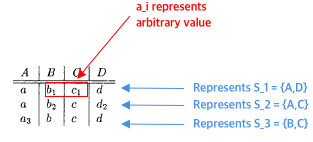
\includegraphics[width=0.7\linewidth]{images/worksheet_13_solution_1.png}
            \end{center}

            \bigskip

            \underline{\textbf{Step 1: $A \to B$}}

            \bigskip

            Set the value $b$ with the same value of $a$ to be the same. (e.g. $b_2 \to b_1$)

            \bigskip

            \begin{center}
            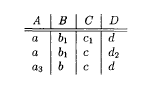
\includegraphics[width=0.7\linewidth]{images/worksheet_13_solution_2.png}
            \end{center}


            \bigskip

            \underline{\textbf{Step 2: $B \to C$}}

            \bigskip

            Set the value $c$ with the same value of $b$ to be the same. (e.g. $b_2 \to b_1$)

            \bigskip

            \begin{center}
            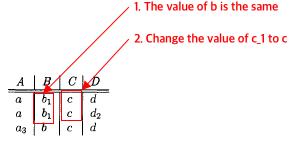
\includegraphics[width=0.7\linewidth]{images/worksheet_13_solution_3.png}
            \end{center}

            \bigskip

            \underline{\textbf{Step 3: $CD \to A$}}

            \bigskip

            Set the value $a$ with the same value of $c$ and $d$ to be the same. (e.g. $a_3 \to a$)

            \bigskip

            \begin{center}
            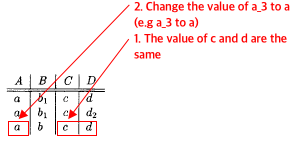
\includegraphics[width=0.7\linewidth]{images/worksheet_13_solution_4.png}
            \end{center}

            \bigskip

            So, we can conclude the join is lossless.

        \end{itemize}

        \item

        \begin{tabular}{|c|c|c|c|c|}
            \hline
            A & B & C & D & E\\
            \hline
            $a$ & $b$ & $c$ & $d_1$ & $e_1$\\
            \hline
            $a_1$ & $b$ & $c$ & $d$ & $e_2$\\
            \hline
            $a$ & $b_1$ & $c$ & $d_2$ & $e$\\
            \hline
        \end{tabular}

        \bigskip

        \underline{\textbf{Step 1 ($AC \to E$):}}

        \bigskip

        \begin{tabular}{|c|c|c|c|c|}
            \hline
            A & B & C & D & E\\
            \hline
            $a$ & $b$ & $c$ & $d_1$ & $\color{red}e$\\
            \hline
            $a_1$ & $b$ & $c$ & $d$ & $e_2$\\
            \hline
            $a$ & $b_1$ & $c$ & $d_2$ & $e$\\
            \hline
        \end{tabular}

        \bigskip

        \underline{\textbf{Step 2 ($BC \to D$):}}

        \bigskip

        \begin{tabular}{|c|c|c|c|c|}
            \hline
            A & B & C & D & E\\
            \hline
            $a$ & $b$ & $c$ & $\color{red}d$ & $\color{red}e$\\
            \hline
            $a_1$ & $b$ & $c$ & $d$ & $e_2$\\
            \hline
            $a$ & $b_1$ & $c$ & $d_2$ & $e$\\
            \hline
        \end{tabular}

        \bigskip

        $a,b,c,d,e$ exists. So by the Chast test, the decomposition of $R(A,B,C,D,E): AC \to E, BC \to D$
        into $\{A,B,C\}$, $\{B,C,D\}$, $\{A,C,E\}$ is lossless.

        \item

        \begin{tabular}{|c|c|c|c|c|}
            \hline
            A & B & C & D & E\\
            \hline
            $a$ & $b$ & $c$ & $d_1$ & $e_1$\\
            \hline
            $a_1$ & $b$ & $c$ & $d$ & $e_2$\\
            \hline
            $a$ & $b_1$ & $c$ & $d_2$ & $e$\\
            \hline
        \end{tabular}

        \underline{\textbf{Step 1 ($A \to D$):}}

        \bigskip

        \begin{tabular}{|c|c|c|c|c|}
            \hline
            A & B & C & D & E\\
            \hline
            $a$ & $b$ & $c$ & $d_1$ & $e_1$\\
            \hline
            $a_1$ & $b$ & $c$ & $d$ & $e_2$\\
            \hline
            $a$ & $b_1$ & $c$ & $\color{red}d_1$ & $e$\\
            \hline
        \end{tabular}

        \underline{\textbf{Step 2 ($D \to E$):}}

        \bigskip

        \begin{tabular}{|c|c|c|c|c|}
            \hline
            A & B & C & D & E\\
            \hline
            $a$ & $b$ & $c$ & $d_1$ & $\color{red}e$\\
            \hline
            $a_1$ & $b$ & $c$ & $d$ & $e_2$\\
            \hline
            $a$ & $b_1$ & $c$ & $\color{red}d_1$ & $e$\\
            \hline
        \end{tabular}

        \bigskip

        \underline{\textbf{Step 3 ($B \to D$):}}

        \bigskip

        \begin{tabular}{|c|c|c|c|c|}
            \hline
            A & B & C & D & E\\
            \hline
            $a$ & $b$ & $c$ & $\color{red}d$ & $\color{red}e$\\
            \hline
            $a_1$ & $b$ & $c$ & $d$ & $e_2$\\
            \hline
            $a$ & $b_1$ & $c$ & $\color{red}d$ & $e$\\
            \hline
        \end{tabular}

        \bigskip

        $a,b,c,d,e$ exists. So by the Chast test, the decomposition of $R(A,B,C,D,E): A \to D, D \to E, B \to D$
        into $\{A,B,C\}$, $\{B,C,D\}$, $\{A,C,E\}$ is lossless.

        \item

        \begin{tabular}{|c|c|c|c|c|}
            \hline
            A & B & C & D & E\\
            \hline
            $a$ & $b$ & $c$ & $d_1$ & $e_1$\\
            \hline
            $a_1$ & $b$ & $c$ & $d$ & $e_2$\\
            \hline
            $a$ & $b_1$ & $c$ & $d_2$ & $e$\\
            \hline
        \end{tabular}

        \underline{\textbf{Step 1 ($A \to D$):}}

        \bigskip

        \begin{tabular}{|c|c|c|c|c|}
            \hline
            A & B & C & D & E\\
            \hline
            $a$ & $b$ & $c$ & $d_1$ & $e_1$\\
            \hline
            $a_1$ & $b$ & $c$ & $d$ & $e_2$\\
            \hline
            $a$ & $b_1$ & $c$ & $\color{red}d_1$ & $e$\\
            \hline
        \end{tabular}

        \bigskip

        \underline{\textbf{Step 2 ($CD \to E$):}}

        \bigskip

        \begin{tabular}{|c|c|c|c|c|}
            \hline
            A & B & C & D & E\\
            \hline
            $a$ & $b$ & $c$ & $d_1$ & $\color{red}e$\\
            \hline
            $a_1$ & $b$ & $c$ & $d$ & $e_2$\\
            \hline
            $a$ & $b_1$ & $c$ & $\color{red}d_1$ & $e$\\
            \hline
        \end{tabular}

        \bigskip

        \underline{\textbf{Step 3 ($E \to D$):}}

        \bigskip

        \begin{tabular}{|c|c|c|c|c|}
            \hline
            A & B & C & D & E\\
            \hline
            $a$ & $b$ & $c$ & $d_1$ & $\color{red}e$\\
            \hline
            $a_1$ & $b$ & $c$ & $d$ & $e_2$\\
            \hline
            $a$ & $b_1$ & $c$ & $\color{red}d_1$ & $e$\\
            \hline
        \end{tabular}

        \bigskip

        So in this case, an example of an instance of $R$ that is not lossless
        is:

        \bigskip

        \begin{tabular}{|c|c|c|c|c|}
            \hline
            Phone ID & Grade & Student Name & Phone \# & Physical Address\\
            \hline
            1 & 89 & John Doe & 111-222-3333 & 123 ABC Street\\
            \hline
            2 & 89 & John Doe & 222-222-3333 & 123 ABC Street\\
            \hline
            1 & 62 & Josh Doe & 111-222-3333 & 123 ABC Street\\
            \hline
            3 & 94 & Frank McKay & 444-555-6666 & 123 ABC Street\\
            \hline
        \end{tabular}

        \bigskip

        \begin{itemize}
            \item $S_1 = \{A,B,C\}$

            \bigskip

            \begin{tabular}{|c|c|c|}
                \hline
                Phone ID & Grade & Student Name\\
                \hline
                1 & 89 & John Doe\\
                \hline
                1 & 62 & Josh Doe\\
                \hline
                2 & 94 & Frank McKay\\
                \hline
            \end{tabular}

            \item $S_2 = \{C,D,E\}$

            \bigskip

            \begin{tabular}{|c|c|c|c|c|}
                \hline
                Student Name & Phone \# & Physical Address\\
                \hline
                John Doe & 111-222-3333 & 123 ABC Street\\
                \hline
                Josh Doe & 111-222-3333 & 123 ABC Street\\
                \hline
                Frank McKay & 444-555-6666 & 123 ABC Street\\
                \hline
            \end{tabular}

            \item $S_3 = \{A,C,E\}$

            \bigskip

            \begin{tabular}{|c|c|c|c|c|}
                \hline
                Phone ID & Student Name & Physical Address\\
                \hline
                1 & John Doe & 1123 ABC Street\\
                \hline
                1 & Josh Doe & 123 ABC Street\\
                \hline
                2 & Frank McKay & 123 ABC Street\\
                \hline
            \end{tabular}

            \item $S_1 \bowtie S_2$

            \begin{tabular}{|c|c|c|c|c|}
                \hline
                Title & Studio Name & President & Year & President Address\\
                \hline
                Toy Story & Pixar & Steve Jobs & 2000 & 123 ABC Street\\
                \hline
                Star Wars & Fox & Lachlan Murdoch & 1977 & Hollywood\\
                \hline
                Star Wars & Fox & Lachlan Murdoch & 1983 & Hollywood\\
                \hline
                Return of the Jedi & Fox & Lachlan Murdoch & 1977 & Hollywood\\
                \hline
                Return of the Jedi & Fox & Lachlan Murdoch & 1983 & Hollywood\\
                \hline
            \end{tabular}

            \item $S_1 \bowtie S_2 \bowtie S_3$

            \begin{tabular}{|c|c|c|c|c|}
                \hline
                Title & Studio Name & President & Year & President Address\\
                \hline
                Toy Story & Pixar & Steve Jobs & 2000 & 123 ABC Street\\
                \hline
                Star Wars & Fox & Lachlan Murdoch & 1977 & Hollywood\\
                \hline
                Star Wars & Fox & Lachlan Murdoch & 1983 & Hollywood\\
                \hline
                Return of the Jedi & Fox & Lachlan Murdoch & 1977 & Hollywood\\
                \hline
                Return of the Jedi & Fox & Lachlan Murdoch & 1983 & Hollywood\\
                \hline
            \end{tabular}

        \end{itemize}


    \end{enumerate}
\end{enumerate}

\end{document}